\section{\texorpdfstring{\ttbar}{TTbar} Background}
\label{sec:bkg_tt}

The \ttbar process contributes about 21\,\% to the total background in our search. We rely on MC to model the process-specific kinematic properties. To that effect, we first verify that the simulation works well in dilepton events, and then correct the MC misidentification rate to match the one in data.

The \ttbar control region is defined by exactly 2 opposite-sign opposite-flavor leptons ($e^\pm \mu^\mp$), at least 1 b-tagged jet above 30\,\GeV, and $\ST > 300\,\GeV$, where \ST is the scalar sum of the lepton transverse momenta, the transverse momenta of jets with $\pt \geq 30\,\GeV$ and $|\eta| \leq 2.4$, and \MET. We use this region to normalize the background prediction. The \MET and \ST distributions are shown in Fig.~\ref{fig:tt2}.

\begin{figure}
\begin{center}
	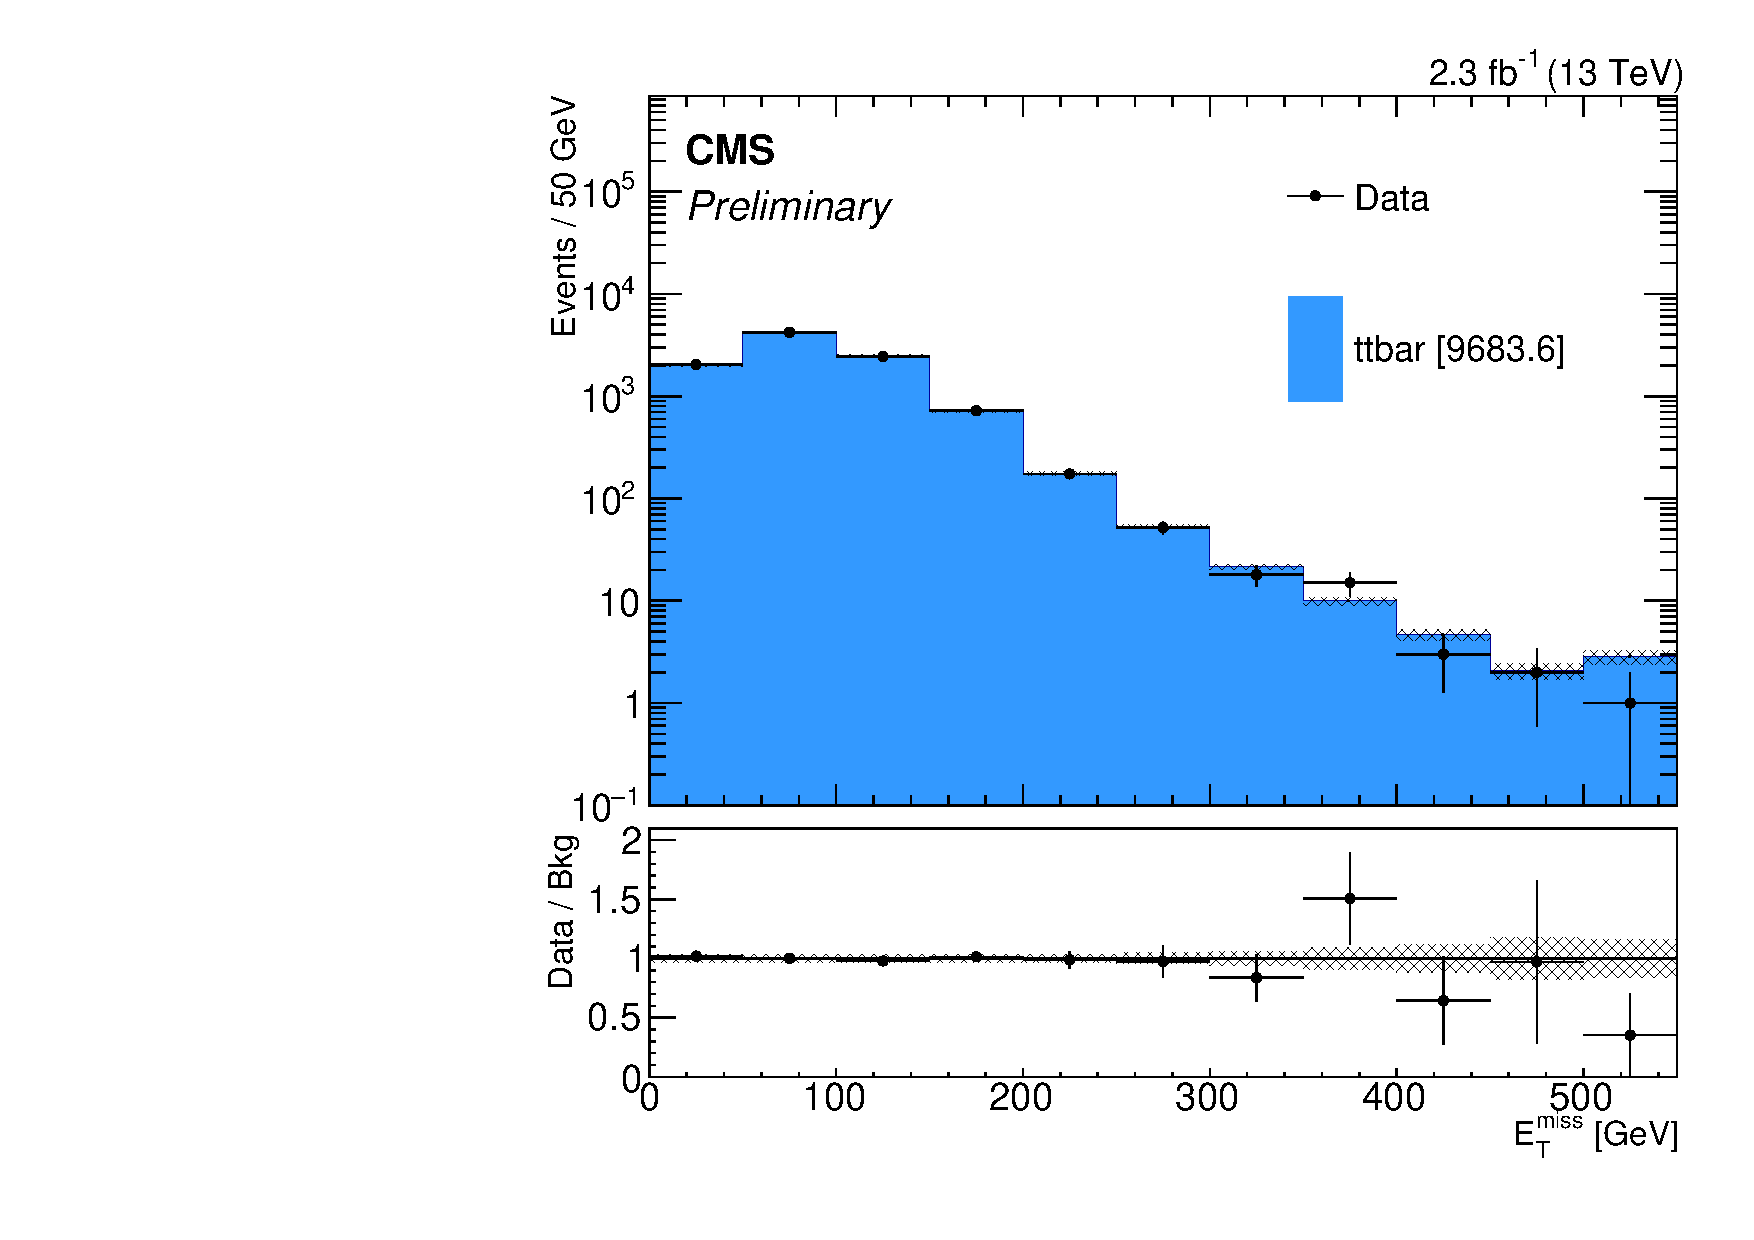
\includegraphics[width=.7\textwidth]{Background/bkg_tt/ttbar_MET_STgt300_afterWeights}
	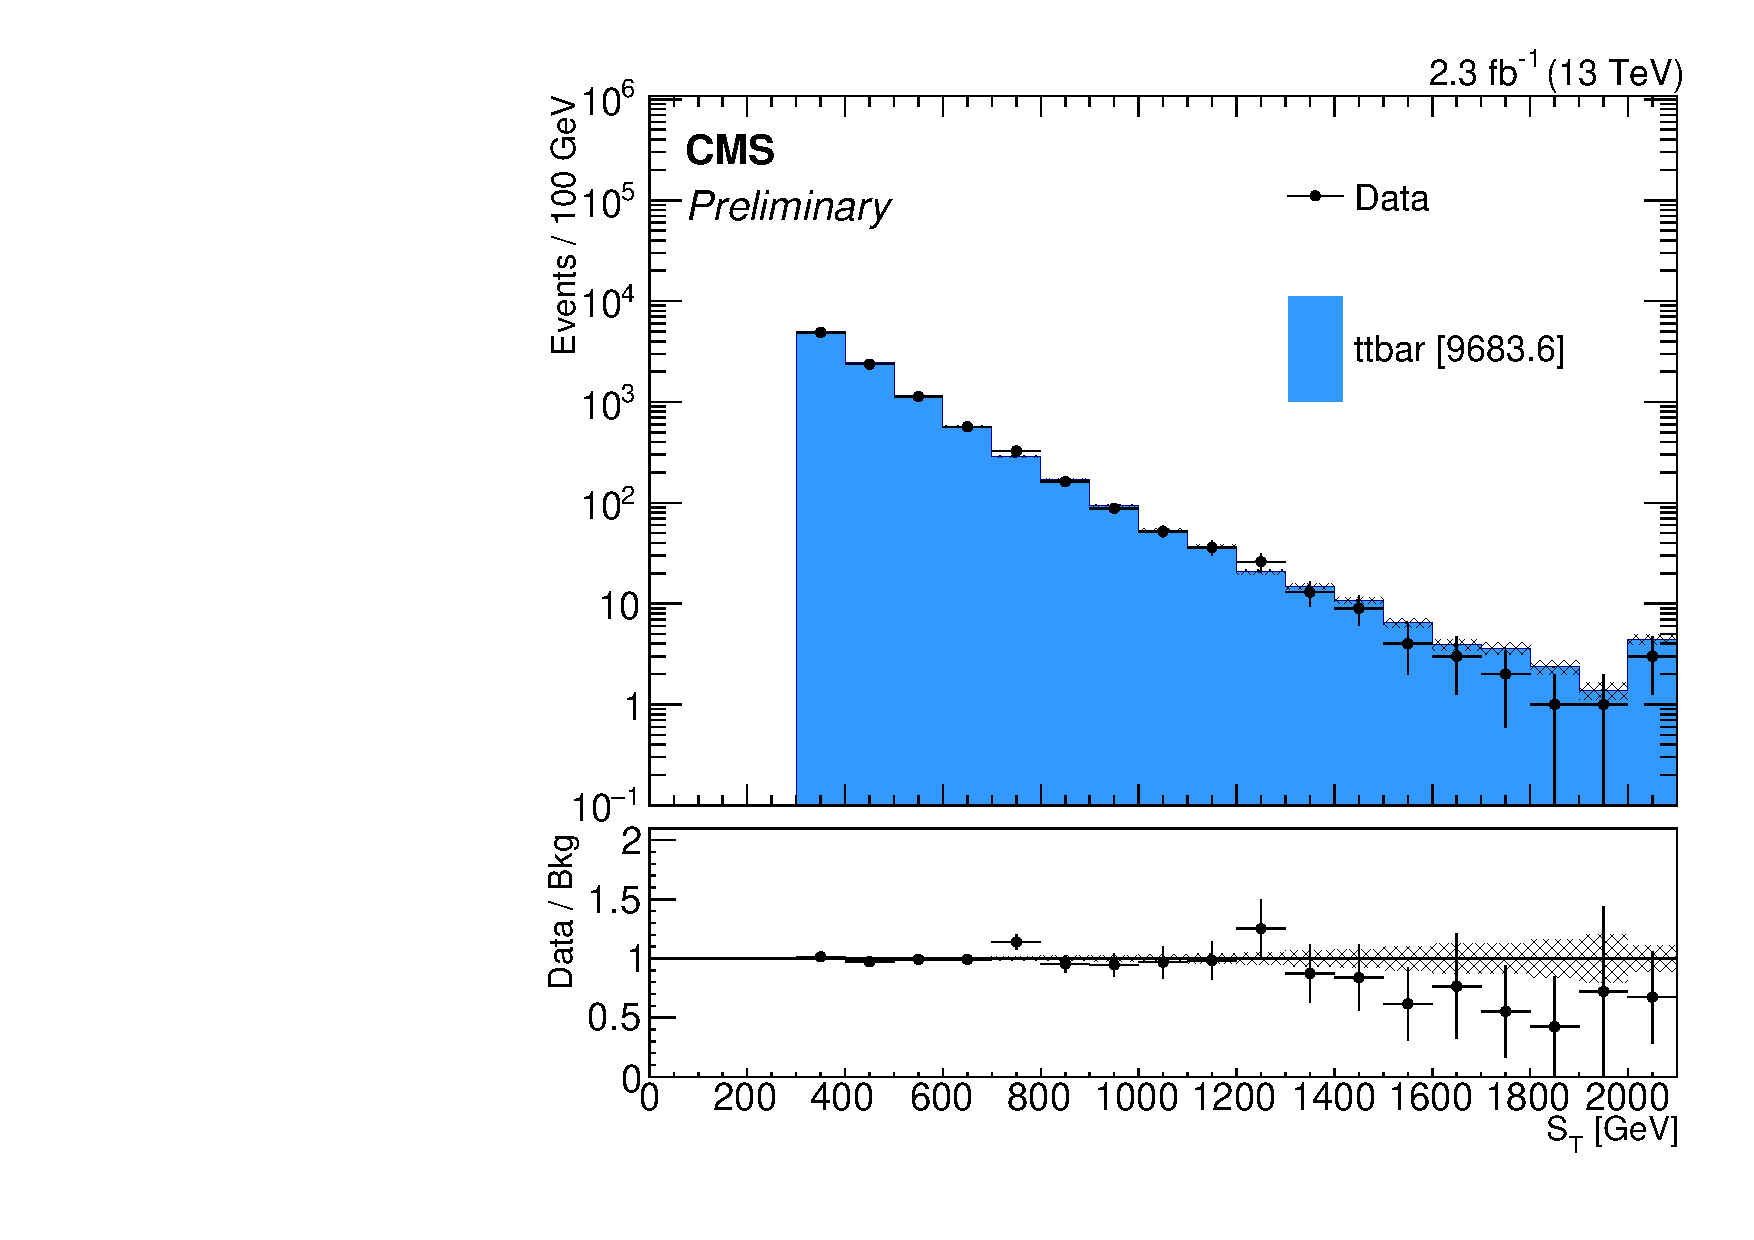
\includegraphics[width=.7\textwidth]{Background/bkg_tt/ttbar_ST_STgt300_afterWeights}
	\caption{\MET (top), and \ST (bottom) distributions in \ttbar-dominated control region (last bin includes overflow). Uncertainties are statistical only.
	\label{fig:tt2}}
\end{center}
\end{figure}

Having established the validity of kinematic aspects of the \ttbar simulation using the dilepton (prompt) sample, we verify that also the rate at which the \ttbar MC produces trilepton events is in agreement with that rate in data. To this end, we measure the lepton misidentification rate in a sample dominated by semi-leptonic \ttbar decays. This sample is selected by requiring one tight muon with $\pt > 30\,\GeV$, 2 jets (from the other top quark), one additional b-tagged jet, and a non-prompt lepton which is most likely misidentified.

We find the \ttbar misidentification rate in data to be $1.5 \pm 0.5\stat$ times the one found in the \ttbar simulation. This indicates that the number of events with misidentified leptons is underpredicted in the \ttbar simulation. We thus use this ratio to correct the number of predicted trilepton events and apply a systematic uncertainty of 50\,\%.
